\chapter{Introduction to the CoreASIM Language, Interpreter, and ICEF}
\label{ch:CoreAsimIntro}

\vspace{-1cm}
\begin{center}
Eduard Hirsch
\end{center}

In this chapter an overview of the used technologies for running the INTERLACE Specification is given. At the beginning a quick start description is provided in order to jump right into the execution of the model.

Further details which are enabling the Abstract State Interacting Machines (ASIM) specifications to be executed are discussed and why this possible in a simple and stable manner.

\section{Quick Start Vagrant}
\label{sec:quick-start-vagrant}

There are two base environments available. One based one docker and one based on vagrant. The focus shifted from the vagrant environment which can be downloaded at github\footnote{https://github.com/InterlaceProject/ASIMVagrantEnvironment} to a docker based version which is explained in section \ref{sec:quick-start-docker}. Nevertheless, for developer preferring vagrant, the setup will be still explained.

The vagrant definition provides a running environment for executing the INTERLACE ASIM definitions. During the provisioning process an ubuntu vagrant box is set up which installs the necessary components on that box. It is cloning and building the ICEF framework\footnote{https://github.com/biomics/icef} as well as the ASIM Specification\footnote{https://github.com/InterlaceProject/ASIMSpec} into the data directory where it is finally ready for usage.

\subsection{Prerequisites}

Download and install the following software products:

\begin{itemize}
	\item Virtual Box: https://www.virtualbox.org/
	\item git: https://git-scm.com/downloads
	\item vagrant: https://www.vagrantup.com/
\end{itemize}

\subsection{Clone Environment}

To clone the ASIM vagrant environment from github into a directory git can be utilized:

\begin{lstlisting}
	git clone https://github.com/InterlaceProject/ASIMVagrantEnvironment.git
\end{lstlisting}

\subsection{Execution}

Once all software components are installed and the vagrant definitions are cloned it is possible to call

\begin{lstlisting}
	execute.sh
\end{lstlisting}

from the main directory in order to let the INTERLACE specifications run. Note: when using Windows it is necessary to start that command within git-bash which needs to run in elevated admin mode (right click $\rightarrow$ start as administrator).

On the very first execution the script is provisioning a virtual machine based on ubuntu by calling \texttt{vagrant up} which may take some time. Consecutive calls will be much faster. A detailed description explaining the precise process is covered in section \ref{sec:env-exec}.

Once the execution is started it will run until it is stopped by pressing \textbf{ctrl + c} or by calling

\begin{lstlisting}
	stop.sh
\end{lstlisting}

from any other console window.

\section{Quick Start Docker}
\label{sec:quick-start-docker}

The docker project at github\footnote{https://github.com/InterlaceProject/ASIMDockerEnvironment} is also based on virtualization like the vagrant environment but emphasizing \textit{Operating System} instead of \textit{Hardware virtualization}\footnote{https://www.docker.com/what-container\#comparing}.

\subsection{Prerequisites}

\begin{itemize}
	\item install docker
	\item install git (including git bash for windows)
\end{itemize}

On Linux machines it is important to add the current user to the docker group in order to manage docker container and images. Otherwise all further explained commands need to be executed as root or with sudo.

For Windows machines use \textit{git-bash} to execute the commands described in the following sections.

\subsection{Before First Execution}

In order to configure the environment it is necessary to call the following script:

\begin{lstlisting}
	./configure
\end{lstlisting}

This will generate a docker container image called \textit{asim} where all the necessary frameworks are build and prepared for execution of the specifications. The ICEF framework as well as the ASIM model specifications are cloned outside of the container to simplify development.

\subsection{Execute Specification}

The container image \textit{asim} created during the configuring step can be started by calling

\begin{lstlisting}
	./execute
\end{lstlisting}

A container started in this way is called \textit{active\_asim} and running all the necessary steps like starting an ICEF manager as well a ICEF brapper to run the ASIM specifications.

Like the vagrant environment a running execution may be stopped by pressing \textbf{ctrl + c}.

\section{Execution Environment Stack}
\label{sec:exec-env-stack}

Independent of the used virtualization techniques a consistent base system is used. So both docker as well as vagrant are provisioning a Linux based operating system using an Ubuntu 16.04 LTS (Long Term Support) distribution.
That consistent, stable and reliable structure will be important later when considerations about provability as well testability come into place. That design provides always the same preconditions and everybody executing or testing against the specifications will receive the same results.

\subsection{Software Stack}
\label{sec:env-exec-stack-software-stack}

The Ubuntu 16.04 LTS distribution is enhanced and updated according to the needs of an ASIM executing machine as well as to the needs of developers working with that virtual system. To be more specific the following components are installed during the provisioning process:

\begin{itemize}
	\item curl $\rightarrow$ Tool for querying REST resources (used for downloading package resources)
	\item nodejs $\rightarrow$ JavaScript engine including the package manager npm (running the Manager Component of ICEF)
	\item build-essential $\rightarrow$ Packages needed to compile a debian based package (used for building the project sources)
	\item maven $\rightarrow$ Java build and packaging tool (used for building the project sources)
	\item vim $\rightarrow$ Well known U/Linux editor (for development purposes)
	\item git $\rightarrow$ Distributed Version Control System (downloading source repositories from GitHub)
	\item Java 8 $\rightarrow$ Programming Language used for coreASIM base system implementation (running ASIM instances)
\end{itemize}

\subsection{Provisioning Process}

The provisioning process can be separated into 3 steps which are executed when \textit{.\/configure} for docker or \textit{vagrant up} for vagrant is called from the command line:

\begin{enumerate}
	\item Download ASIMSpec and ICEF from GitHub
	\item Install of software packages mentioned in section \ref{sec:env-exec-stack-software-stack}
	\item Build ICEF framework and prepare virtual machine for execution
\end{enumerate}

For development purposes the ASIMSpec as well as the ICEF framework are cloned into directories which are available from the host machine and the virtual guest machine. This is necessary because then it is possible to directly edit the source or debug from outside and execute the code from within the container. Consequently it is not necessary to copy the code into the container when changes where done.

\todo{move to exec stack?}
For \textbf{Vagrant} shared folder is configured over the vagrant file

\begin{lstlisting}
	config.vm.synced_folder "./data", "/vagrant-data"
\end{lstlisting}

saying that on the host system the folder \textit{data} is used and on the guest system a folder \textit{vagrant-data} is mounted which are shared and thus containing the same content. Additionally during provisioning a symbolic link in the home directory is created called project (\textit{/home/ubuntu/project}) which is linking the mounted root folder /vagrant-data.

When the virtual machine is stopped the data directory on the host is kept and can be still manipulated or executed (of course only if the framework dependencies are installed on the host as well).

For \textbf{Docker} we need to first clone all GitHub sources to the host machine and can only then share the files into the guest container by using the command line option "-v"

\begin{lstlisting}
	docker run -v "$1/ASIMSpec:/home/ASIMSpec" \
	           -v "$1/icef:/home/icef" \
	           --name active_asim -it asim /$2
\end{lstlisting}

This line is part of the script \textit{scripts/runDocker.sh}. \$1 here stands for the local directory of the environment and \$2 will be explained later in section \ref{sec:env-exec-stack-exec-stack}. Important to note is that the \textit{ASIMSpec} folder of the host machine is shared into \textit{/home/ASIMSpec} of the docker container and the \textit{icef} directory is shared into \textit{/home/icef}.

\subsection{Execution}
\label{sec:env-exec-stack-exe}

The execution stack in figure \ref{fig:icef-intro-asim} shows where a ICEF specification is transmitted to for it to be executed. The details will be covered in section \ref{sec:icef-intro}. In this part of the document, however, we will take a look at how and which services are started.

Due to limitations of the ICEF framework it is currently not possible to cleanly shut down a running ICEF simulation with several running ASIM instances. Therefore both environments have to start and stop all services for every execution in order to grant a correct execution set-up.

Both environments offer a script (\textit{execute(.sh)}) to be called from the host system and one from within the virtualized machine (\textit{executeASIMSpec.sh/executeOnGuest.sh}). Whereas the script on the virtualized system only differ in directory references the outside scripts are need to handle different things as one script is dealing with docker and the other with vagrant.

In detail Docker can immediately start the servers and run the script inside the container whereas vagrant needs add an additional step if the virtual machine is not up and running yet. Thus vagrant

\begin{enumerate}
	\item is trying to start the server processes and submit the specifications
	\item if the first step failed is checking for the virtual machine if it is running and if not it tries to restart the virtual machine
	\item if the restart has been successful the first step will be retried.
\end{enumerate}

When now focusing on the first step which is basically the same on both environments it can be discussed in detail how the process is continued. So on the guest system we are first running a so called \textit{CASIMA} which is short hand for coreASIM-Manager \ref{TODO}. This manager takes care about ASIM states, scheduling and also deals as messaging backbone.

\todo{Brapper, https://github.com/biomics/icef}

\subsection{Development}

\todo{do we need?}

\section{ICEF - The Interaction Computing Execution Framework}
\label{sec:icef-intro}

The interaction framework is wrapping the original coreASM framework in order to extend it and giving it the capabilities to execute concurrent and distributed. It has been developed in a project called BIOMICS and financed by the European Commission.

This wrapping took place on three levels:

First the interpreter coreASM had to be extended supporting additional languages primitives as well as communications features. Here BSL replaces ASM as a new language having a new interpreter coreASIM.

Second a place has been created were the now so called Abstract State Interaction Machines (ASIMs) take over and are able to execute in parallel. This environment is called Brapper (short for BIOMICS Wrapper).

Third a central server called manager takes care handling distributed Brapper instances dealing with message and scheduling issues.

Technology wise coreASIM changes the coreASM implementation in Java. Brappers are written in Java as well but the managers are coordinating the Brappers using nodejs.

\subsection{Framework Stack}

\begin{figure}[htbp]
  \centering
  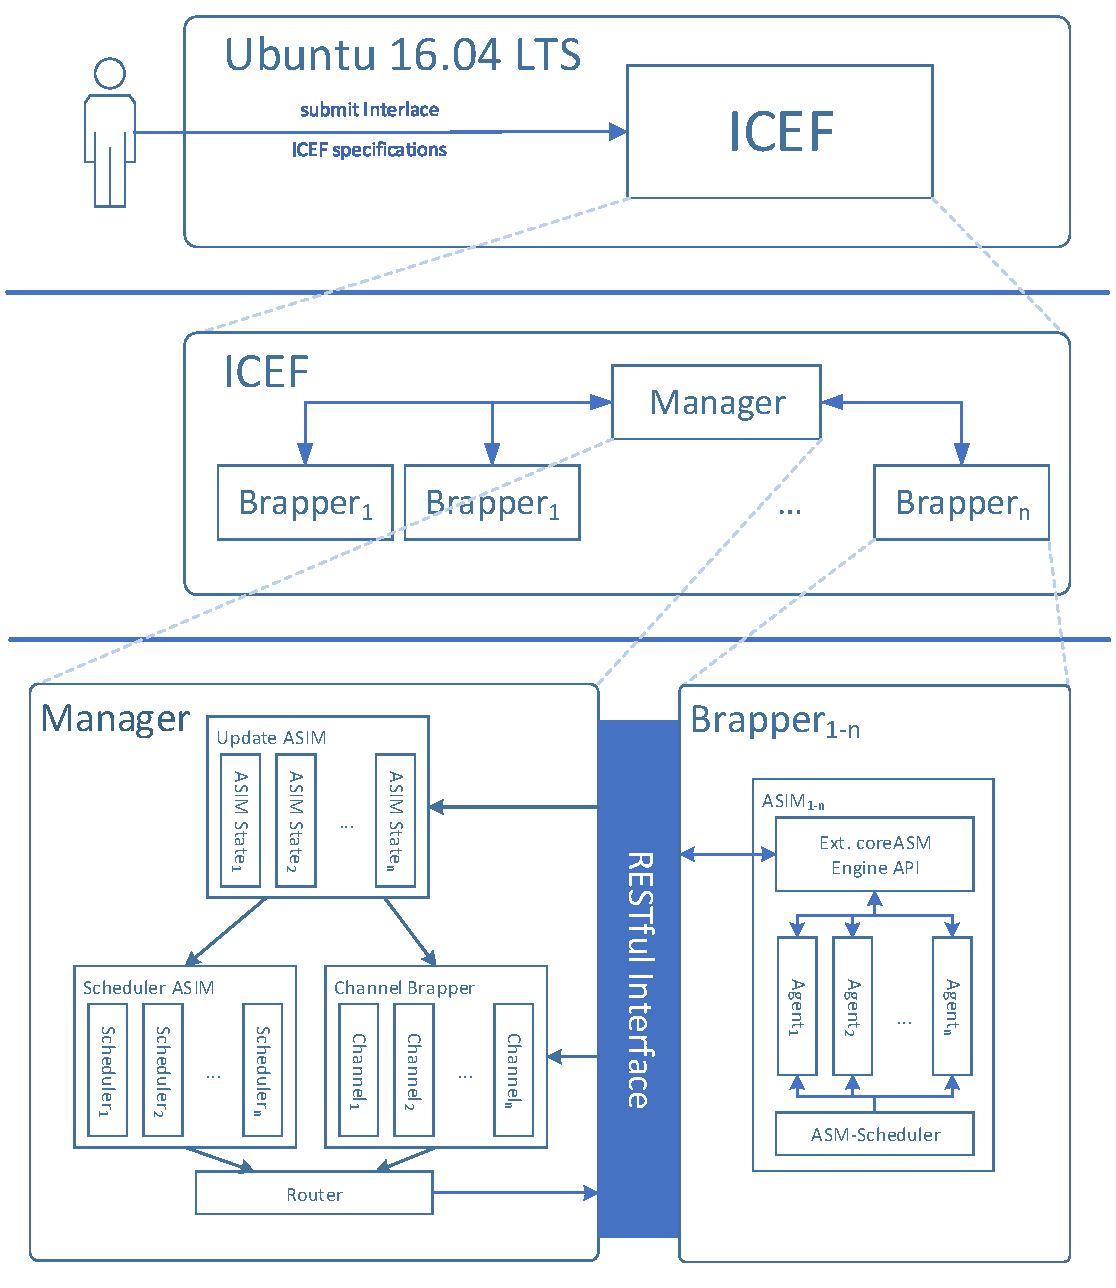
\includegraphics[width=0.9\textwidth, clip, trim=1mm 1mm 1mm 1mm]{Figures/environment_asim}
  \caption{ASIM Execution Environment Overview}
  \label{fig:icef-intro-asim}
\end{figure}


\section{coreASIM}

\section{Interpreter}

\section{INTERLACE Model Execution Environment}
\label{sec:env-exec}

\section{keep for later usage}
\todo{section remove later}
What will happen:
\begin{itemize}
	\item On the very first execution the script is provisioning a virtual machine based on ubuntu by using vagrant up
	\item If the virtual machine is not yet running it tries to start the virtual machine.
	\item If the VM is finally running the script data/execute.sh is called on the guest vm.
\end{itemize}

The actual execution is running inside of the Virtual Machine:

The script data/execute.sh starts the icef manager as well as one brapper. Then it is submitting the specification (run.icef) located in data/ASIMSpec/ to the manager. When done the script is waiting for a stop command or may also be stopped using \textbf{ctrl + c}.

\todo{sections structure, text}